%fig1


% Figure 3
\begin{figure}[H]
\begin{center}
   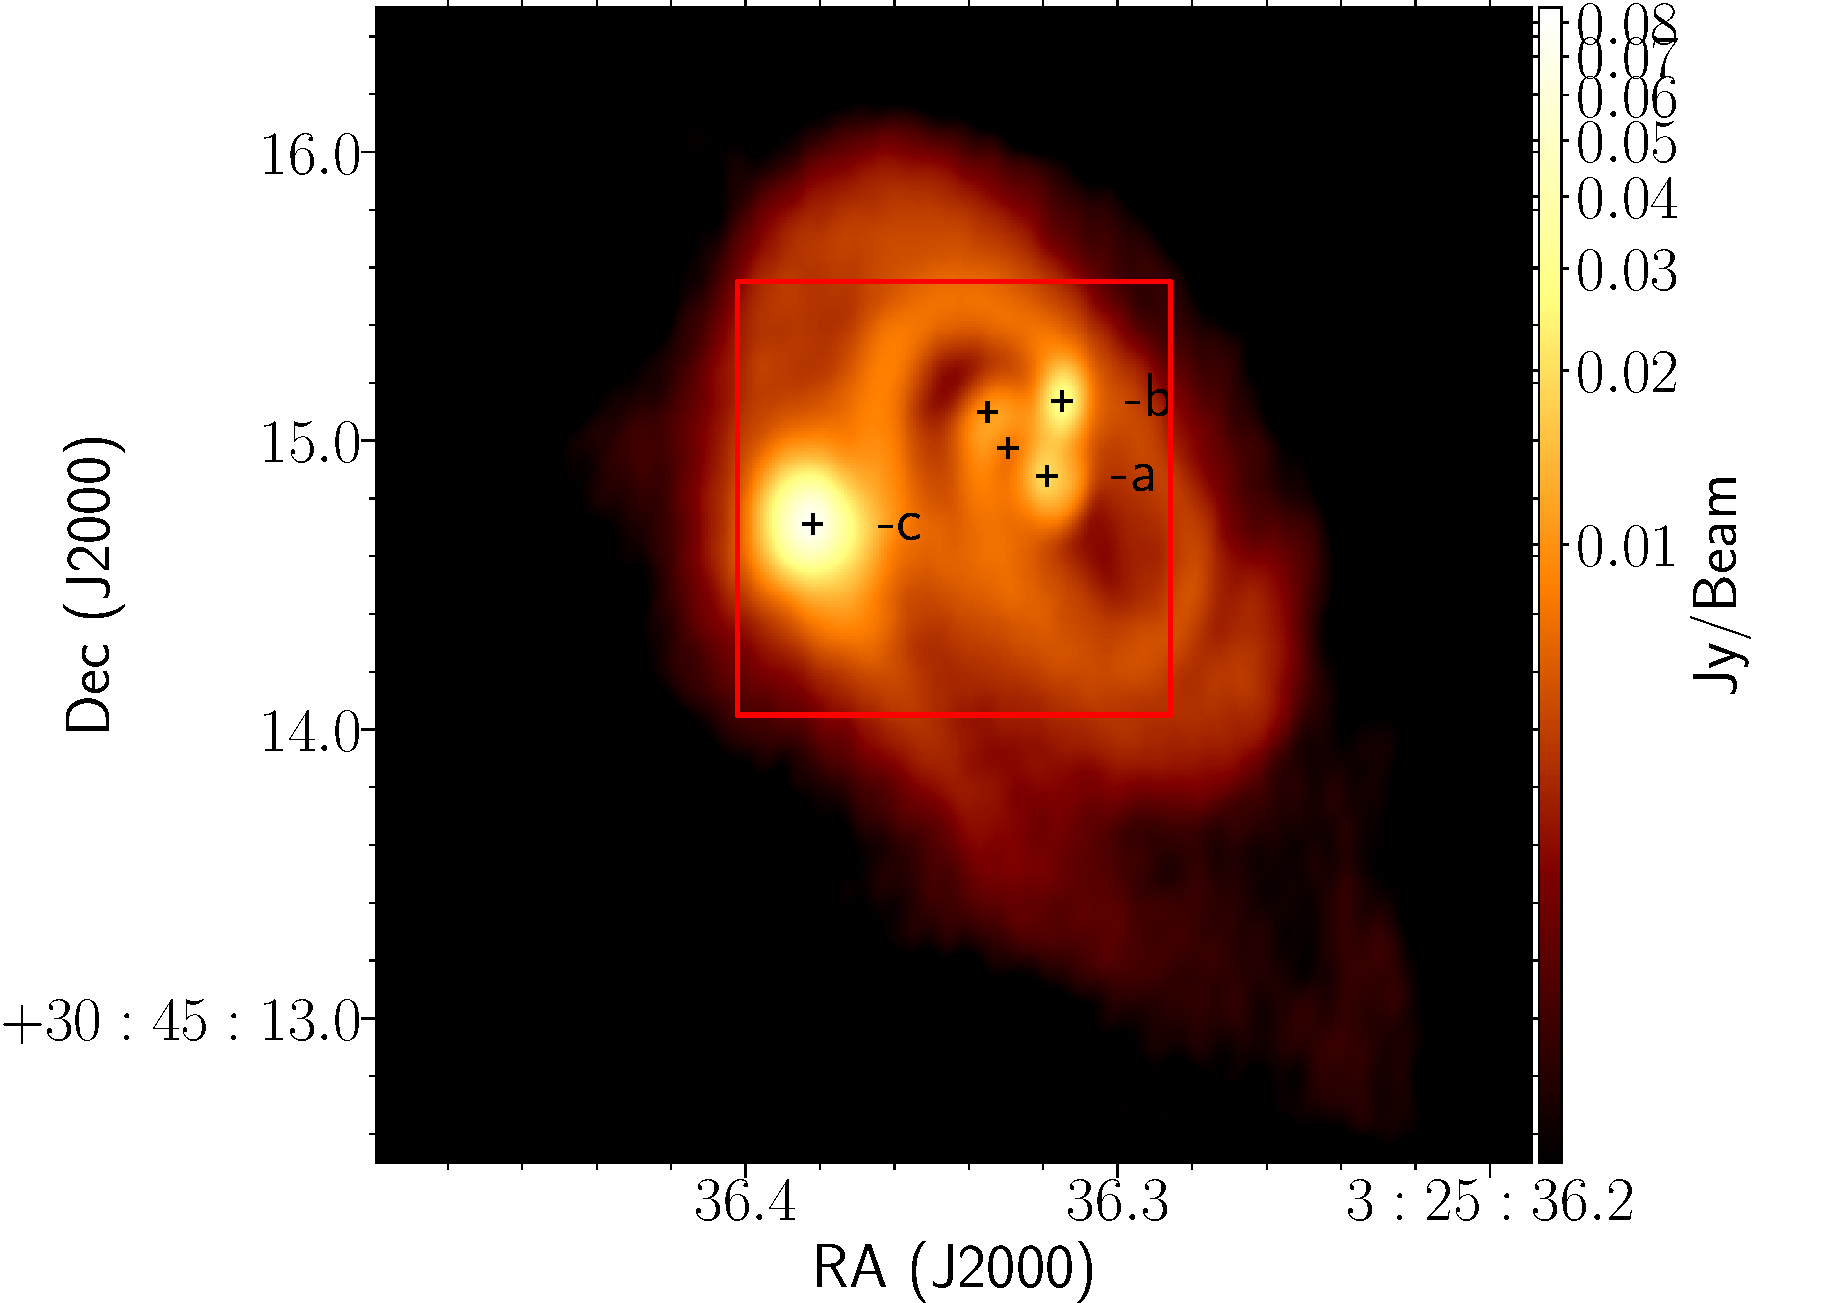
\includegraphics[width=0.49\textwidth]{img/L1448IRS3B_cont_robust05triplet_uc_forpos.pdf} % cont
   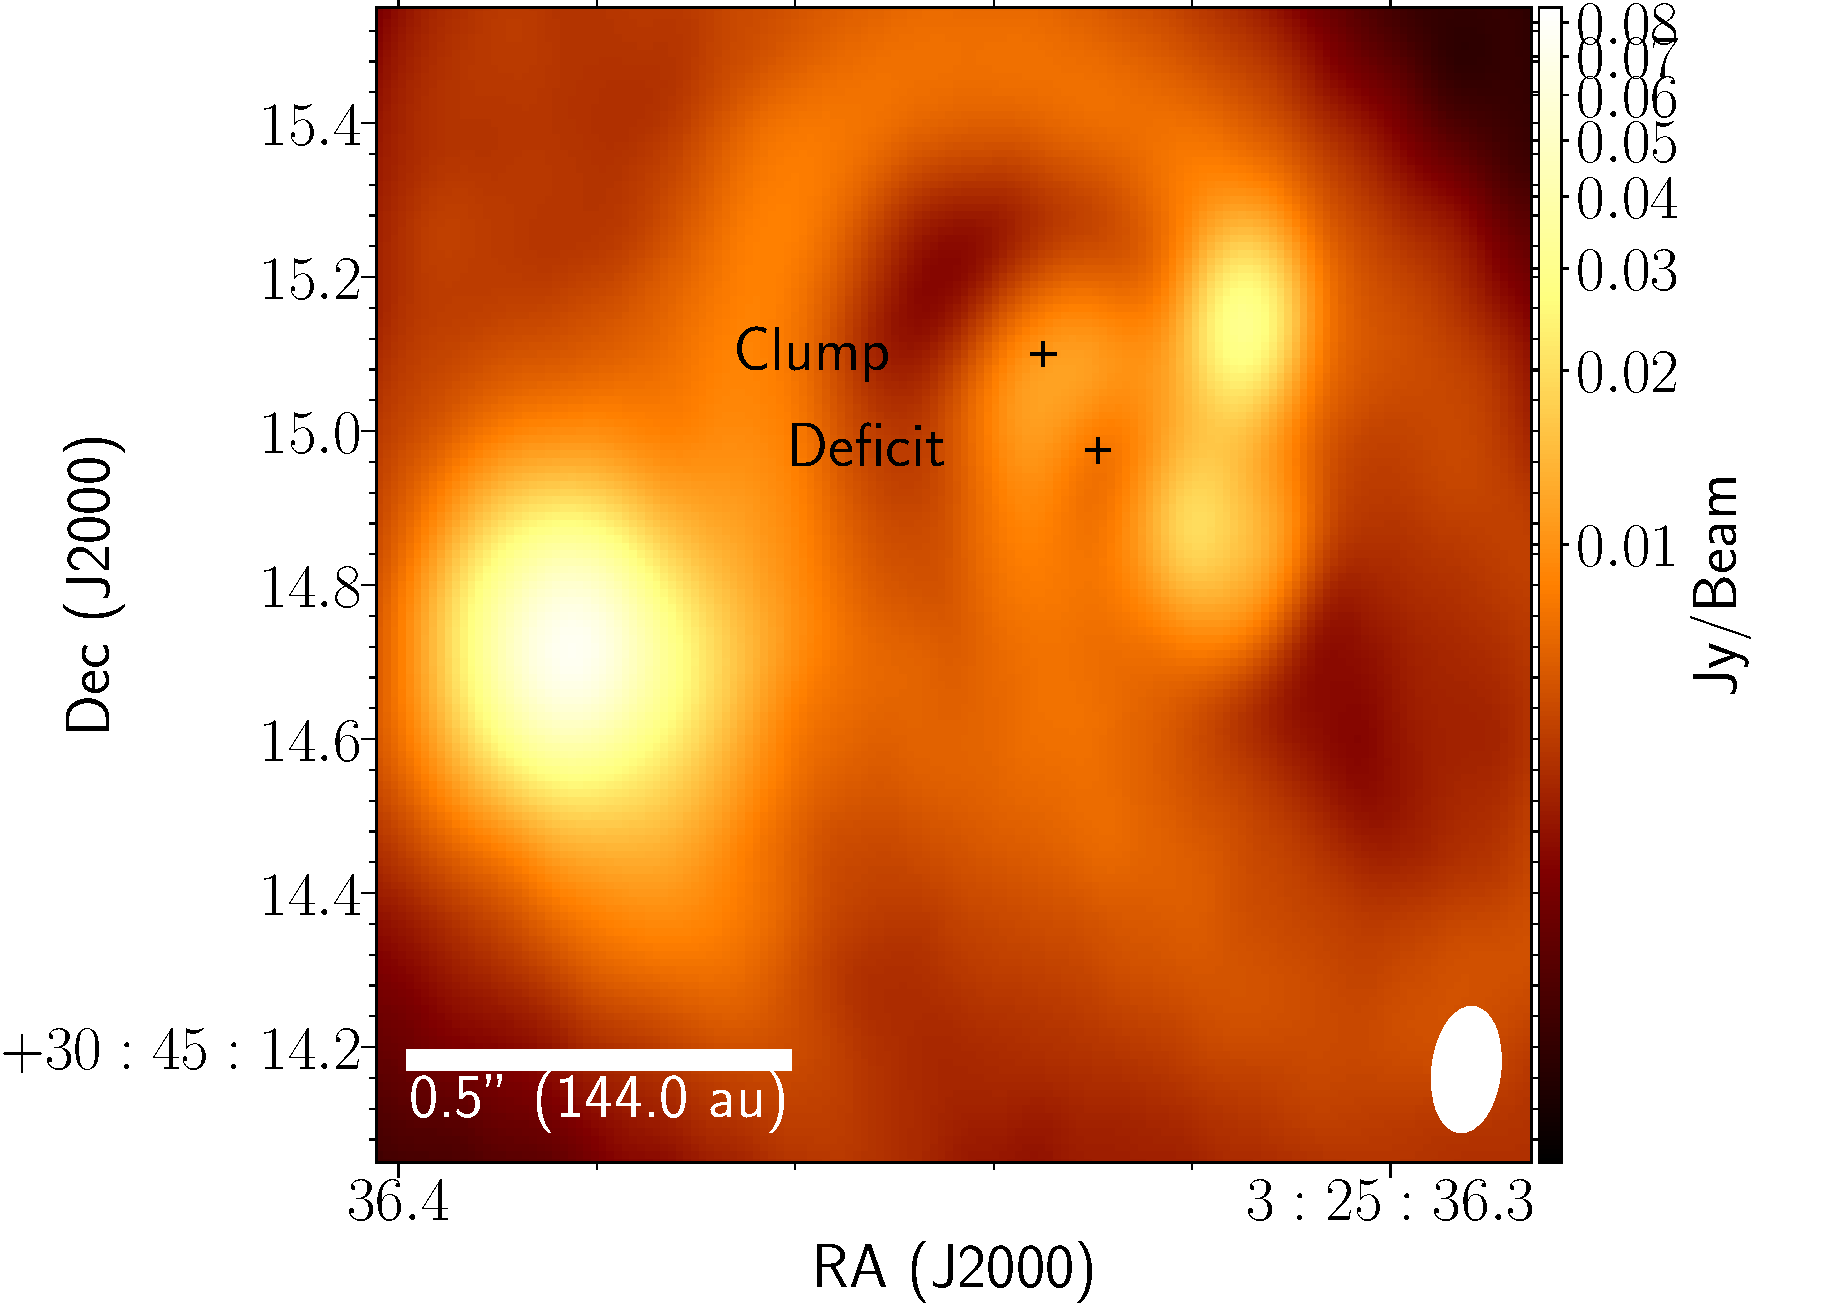
\includegraphics[width=0.49\textwidth]{img/L1448IRS3B_cont_robust05triplet_uc_positions.pdf} % cont
\end{center}
   \caption{ALMA 879~\micron\space continuum observations of the triple protostellar system L1448 IRS3B. The left colored image is zoomed in on IRS3B. The inner binary is separated by 0\farcs25 (75~AU) and has a circum-binary disk with spiral structure and the tertiary is separated from the binary by \ab0\farcs8 (230~AU) within one of the arms. The ``protostars'' are the continuum positions previously discovered in \citet{2016Natur.538..483T}, while the ``clump'' is a new feature, resolved in these observations. The ``deficit'' indicates the location of depression of flux between IRS3B-a and the ``clump''. This is discussed in Section~\ref{sec:dcont}. The beam size of each panel is shown in lower right (\contbeam\space using Briggs Robust parameter of 0.5).}\label{fig:zoomincont}
\end{figure}


\begin{figure}[H]
  \begin{center}
   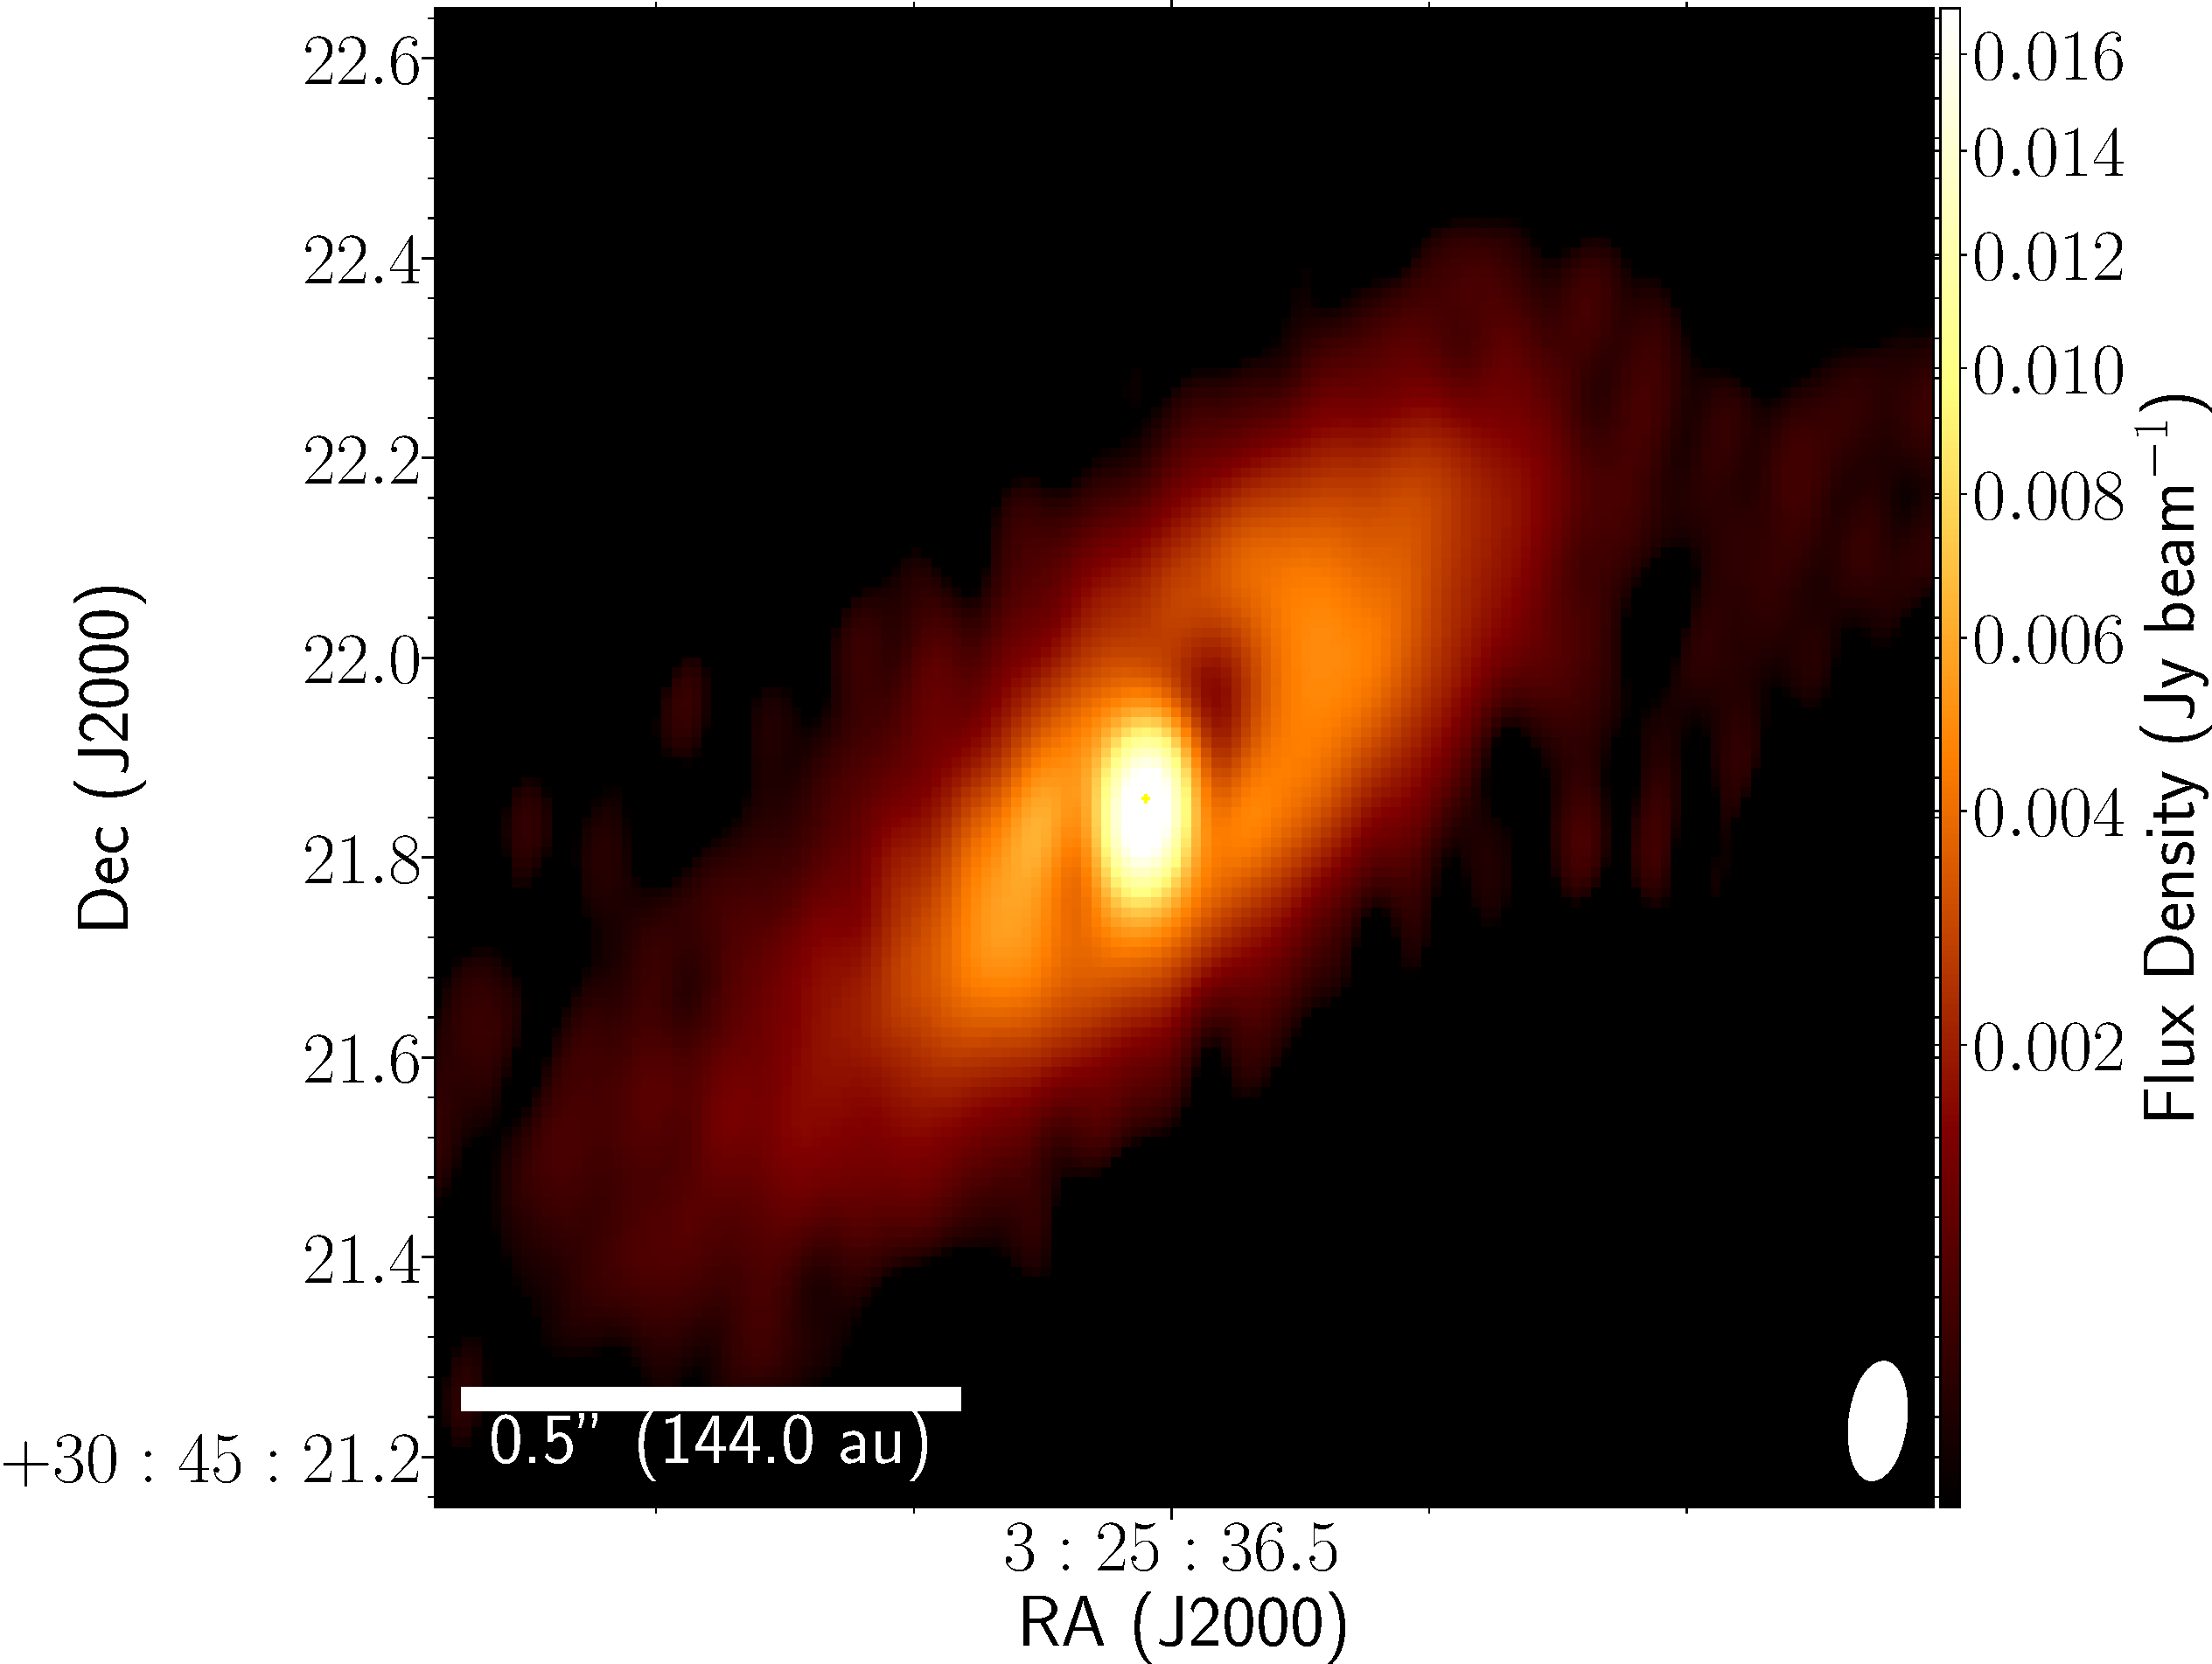
\includegraphics[width=0.48\textwidth]{img/L1448IRS3B-cont-irs3a-highres.pdf} % co
   \end{center}
   \caption{Continuum (879~\micron) image of IRS3A, reconstructed with the \textit{superuniform} weighing scheme, half of the cell size, and zoomed 2x from the images in Figure~\ref{fig:zoomincont}\space to highlight the possible spiral substructure.} \label{fig:widesuperuniform}
\end{figure}


% Figure 2
\begin{figure}[H]
\begin{center}
   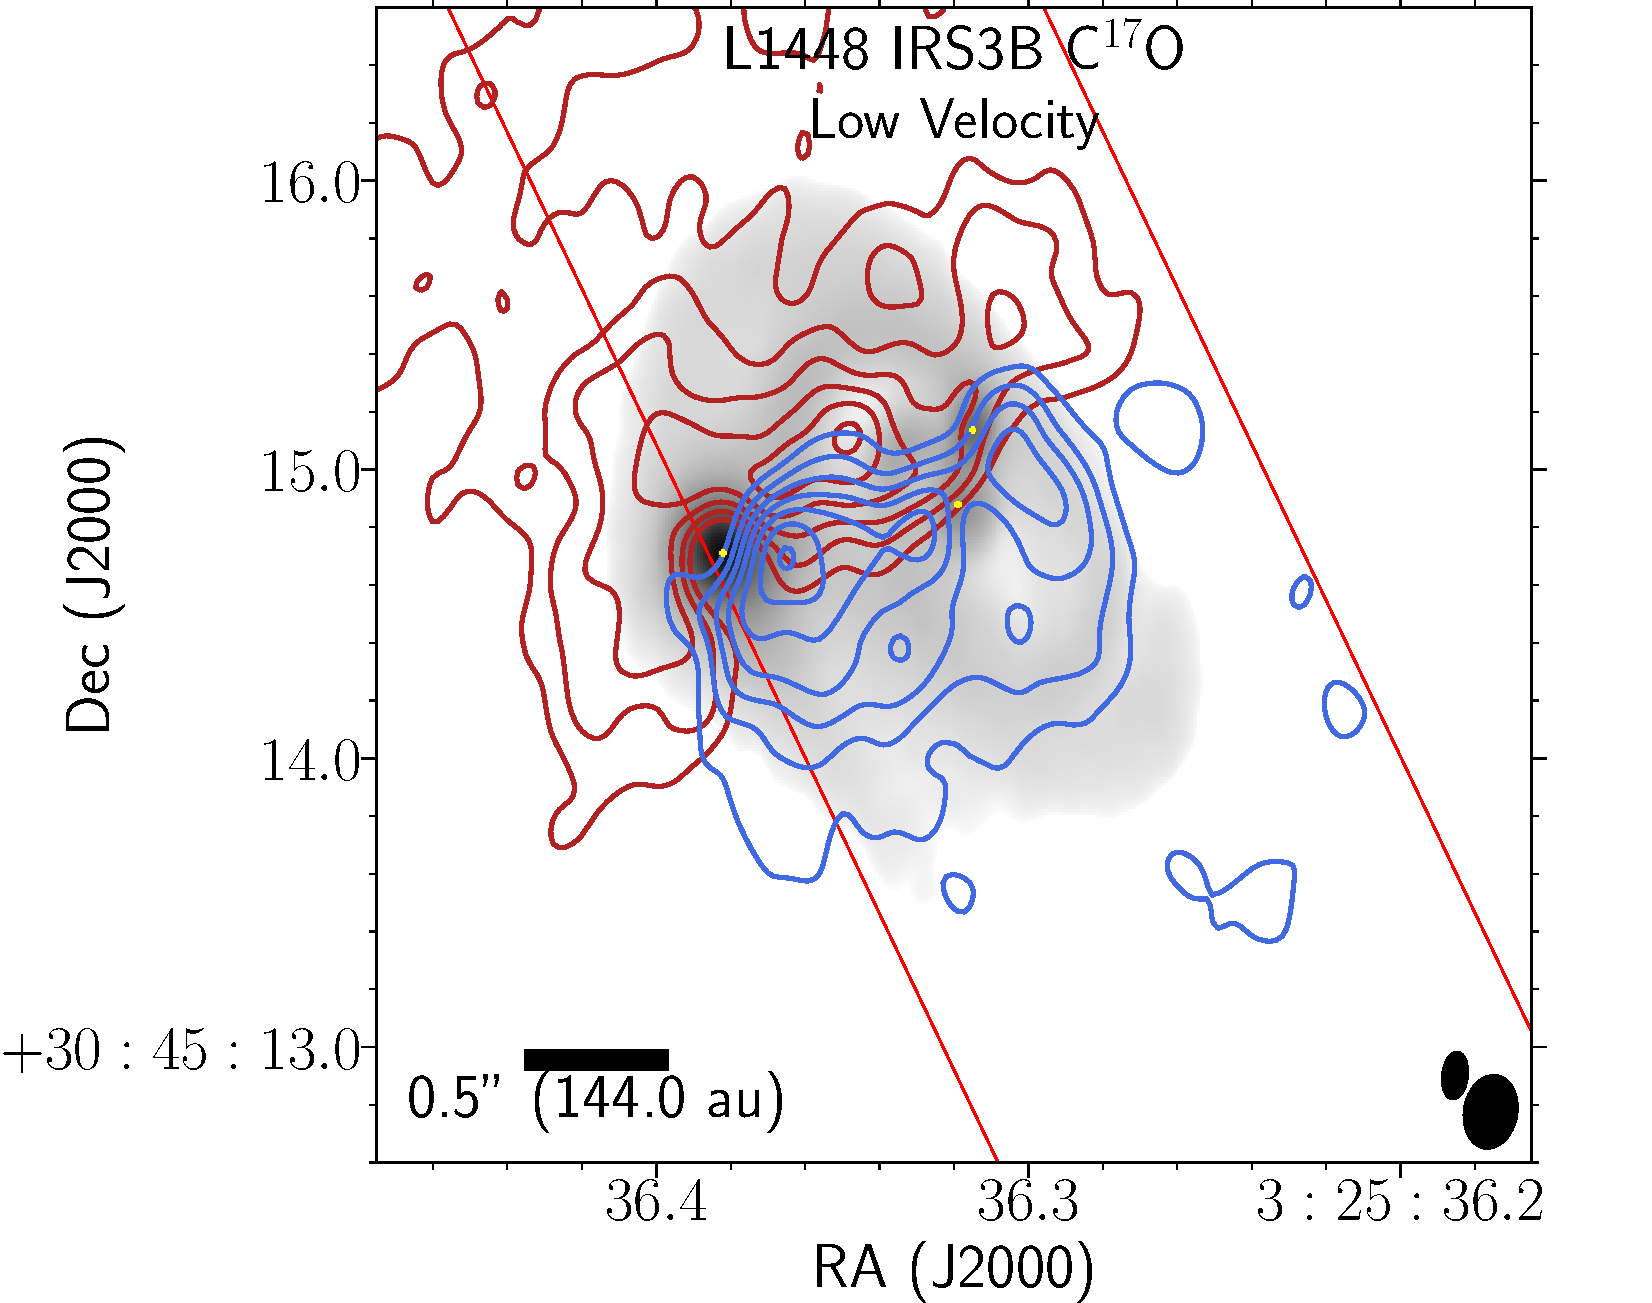
\includegraphics[width=0.33\textwidth]{img/L1448IRS3B_C17O_image_taper1500k__splitMoments_low.pdf} 
   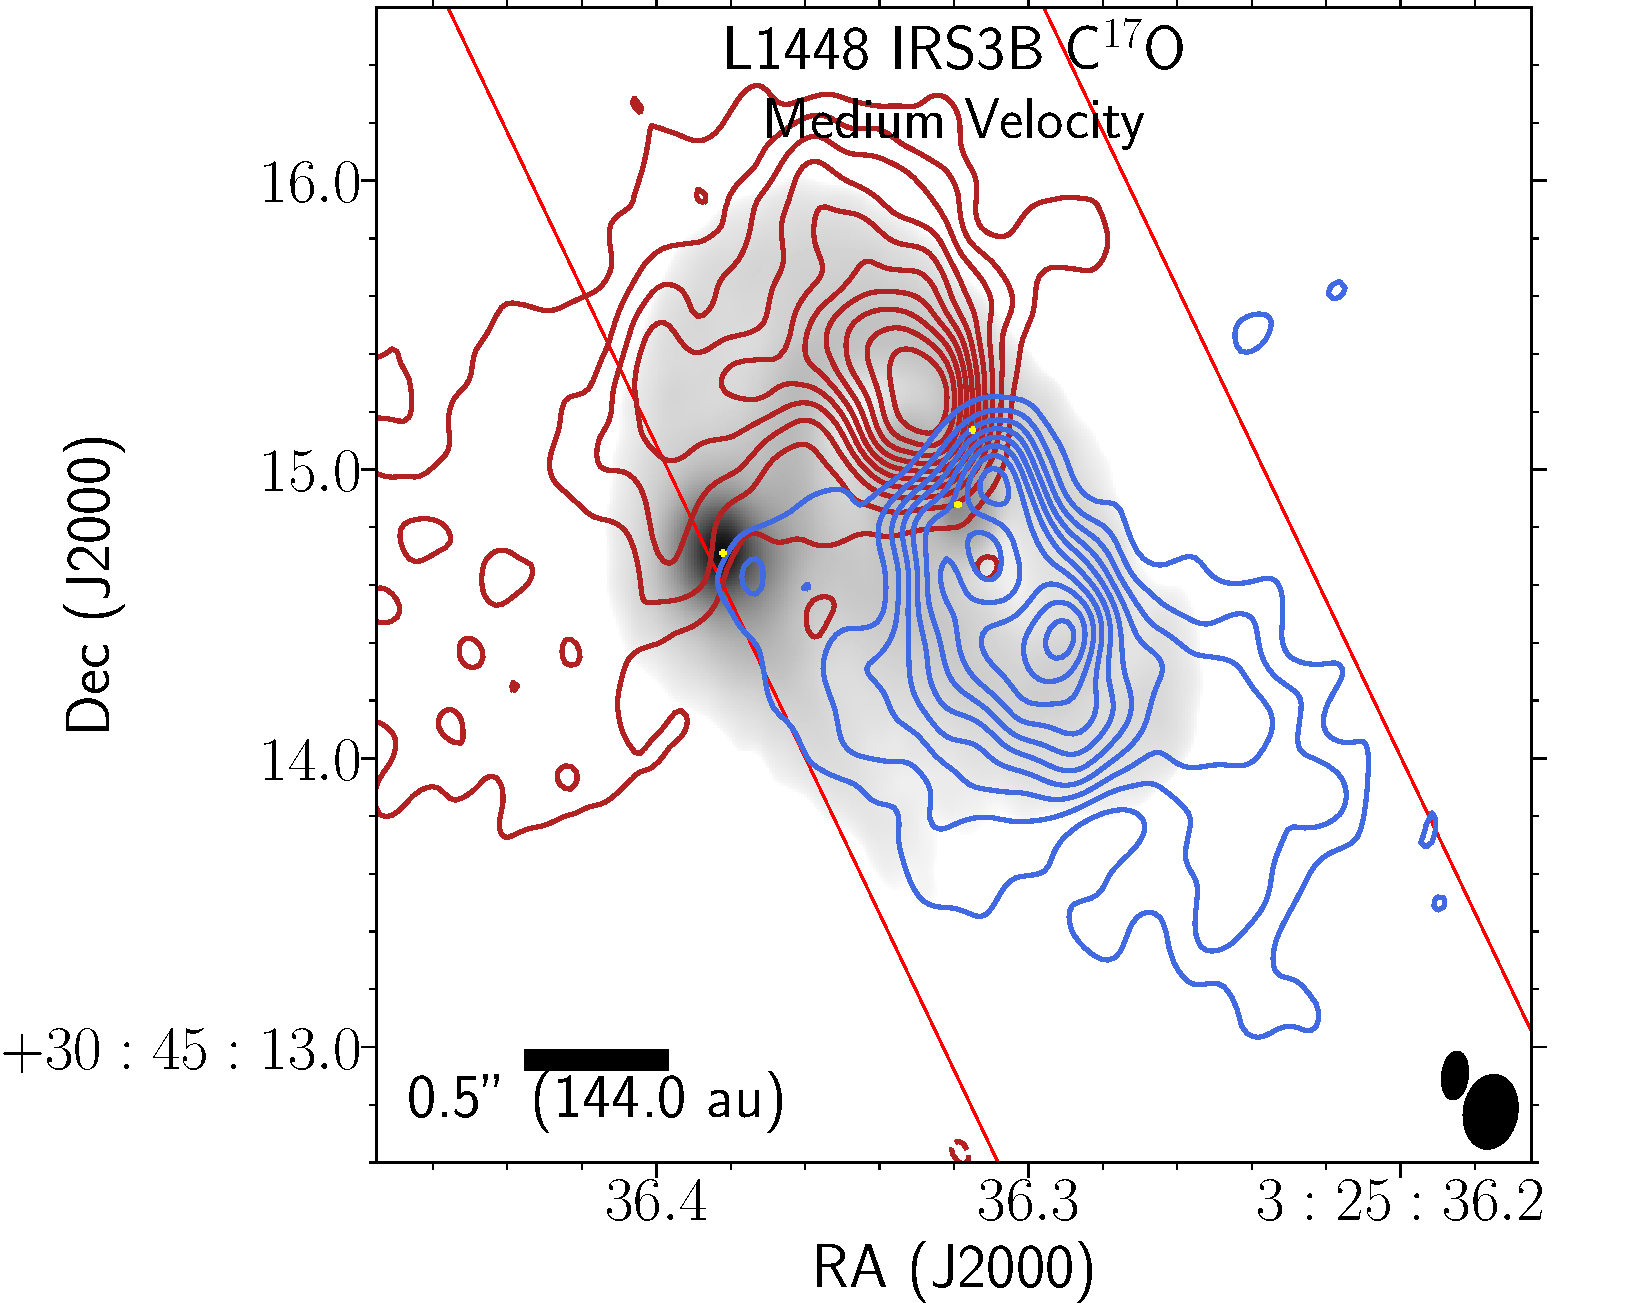
\includegraphics[width=0.33\textwidth]{img/L1448IRS3B_C17O_image_taper1500k__splitMoments_med.pdf} 
   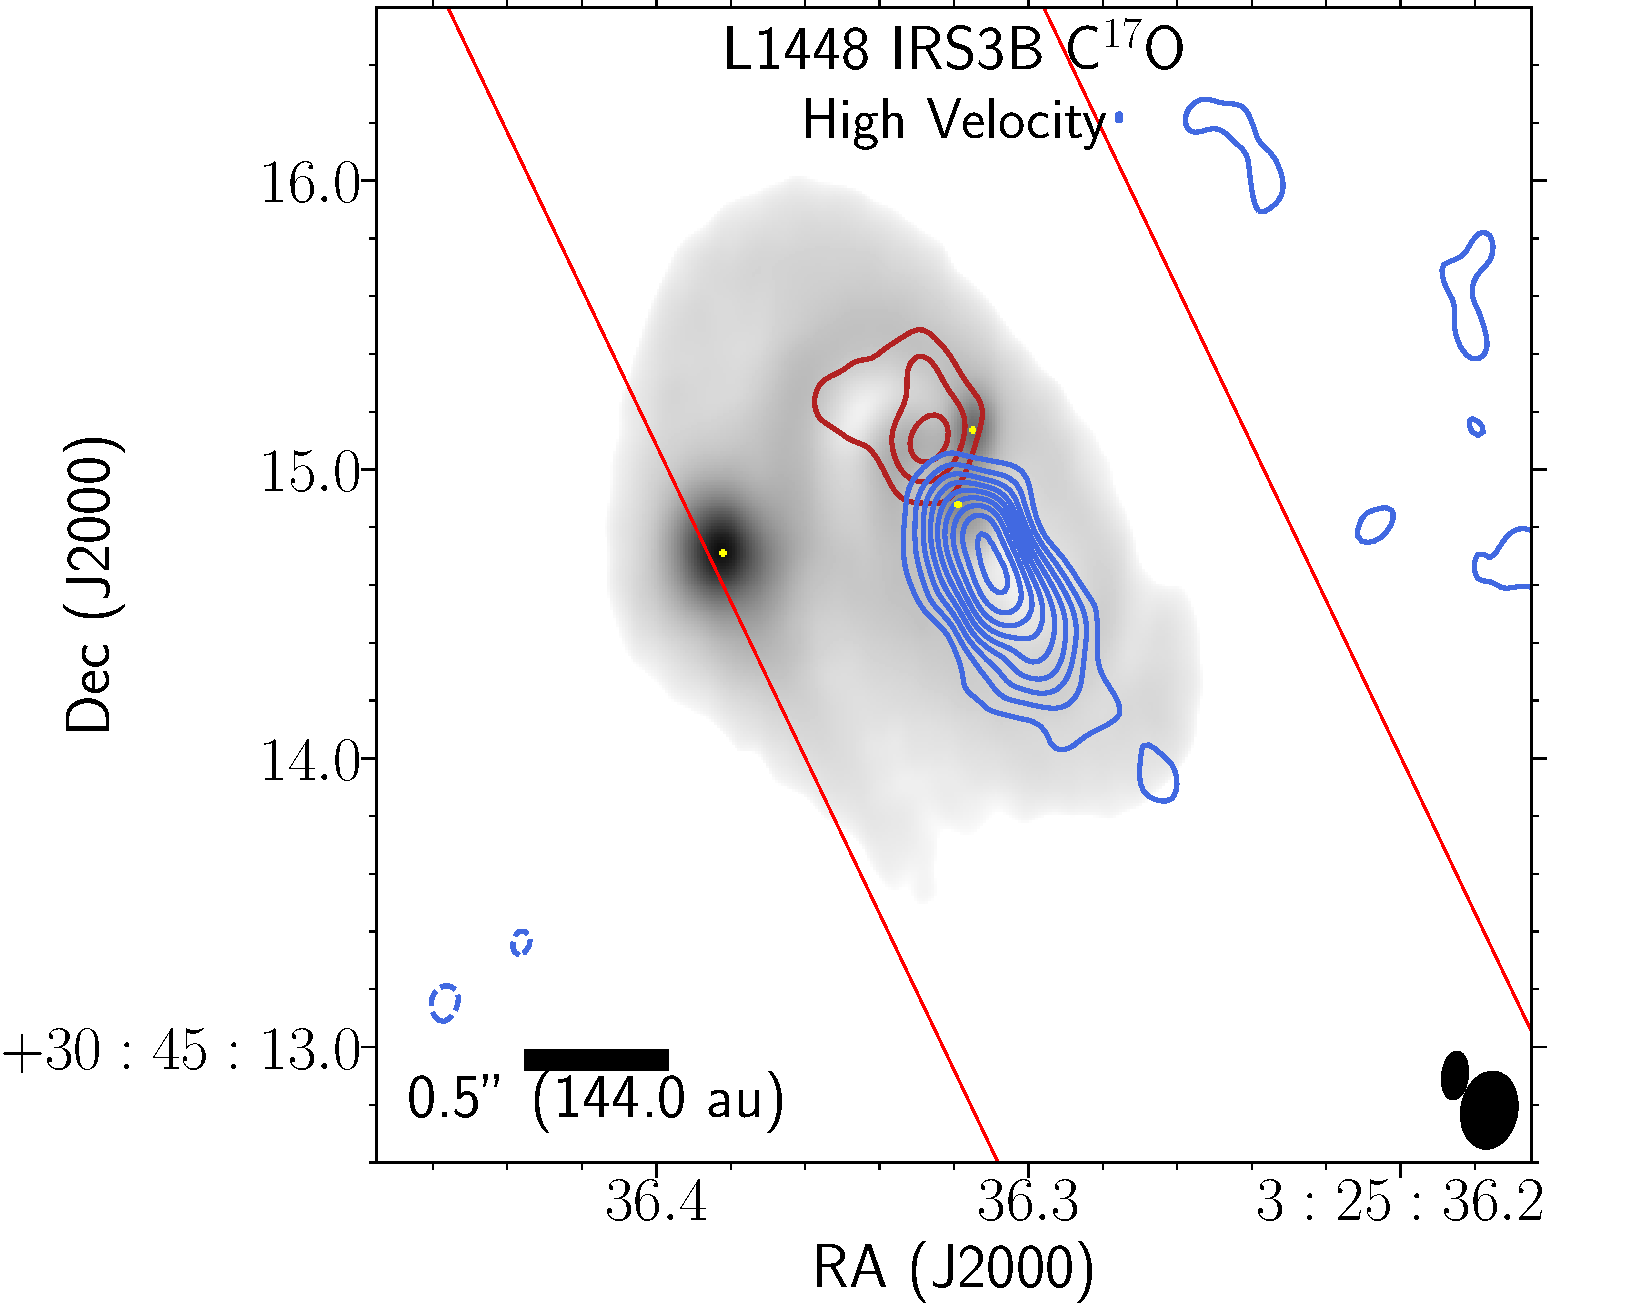
\includegraphics[width=0.33\textwidth]{img/L1448IRS3B_C17O_image_taper1500k__splitMoments_high.pdf}  % c17o
\end{center}
   \caption{\cso\space integrated intensity maps (herein moment 0 map) towards IRS3B over a selected range of velocities overlayed on continuum (grayscale). The \cso\space emission traces the rotating gas within the disk via Doppler-shifted emission. The panels correspond to low, medium, and high velocity ranges.% Negative contours are not present in these moment 0 maps; however, at the location of IRS3B-c, there is strong absorption that is evident in the high spectral resolution data cube, but is not represented here. 
   The red lines indicate the region extracted for PV diagram, along the position angle of the major axis. \textbf{Low Velocity:} Velocity range starts at 4.68$\rightarrow$5.67~\kms (3.58$\rightarrow$4.68~\kms) and contours start at 8(8)$\sigma$ and iterate by 3(3)$\sigma$ with the 1$\sigma$~level starting at 0.0023(0.0025)~Jy~beam$^{-1}$ for the red(blue) channels respectively. \textbf{Medium Velocity:} Velocity range starts at 5.67$\rightarrow$6.66~\kms (2.48$\rightarrow$3.58~\kms) and contours start at 3(5)$\sigma$ and iterate by 3(3)$\sigma$ with the 1$\sigma$~level starting at 0.002(0.0016)~Jy~beam$^{-1}$ for the red(blue) channels respectively. \textbf{High Velocity:} Velocity range starts at 6.66$\rightarrow$7.65~\kms (1.27$\rightarrow$2.48~\kms) and contours start at 5(5)$\sigma$ and iterate by 3(3)$\sigma$ with the 1$\sigma$~level starting at 0.0018(0.0012)~Jy~beam$^{-1}$ for the red(blue) channels respectively. The \cso\space synthesized beam (\csobeam) is the bottom-right most ellipse on each of the panels and the continuum synthesized beam (\contbeam) is offset diagonally.}\label{fig:irs3bc17omoment}
\end{figure}




% Figure 8
% irs3a
\begin{figure}[H]
\begin{center}
   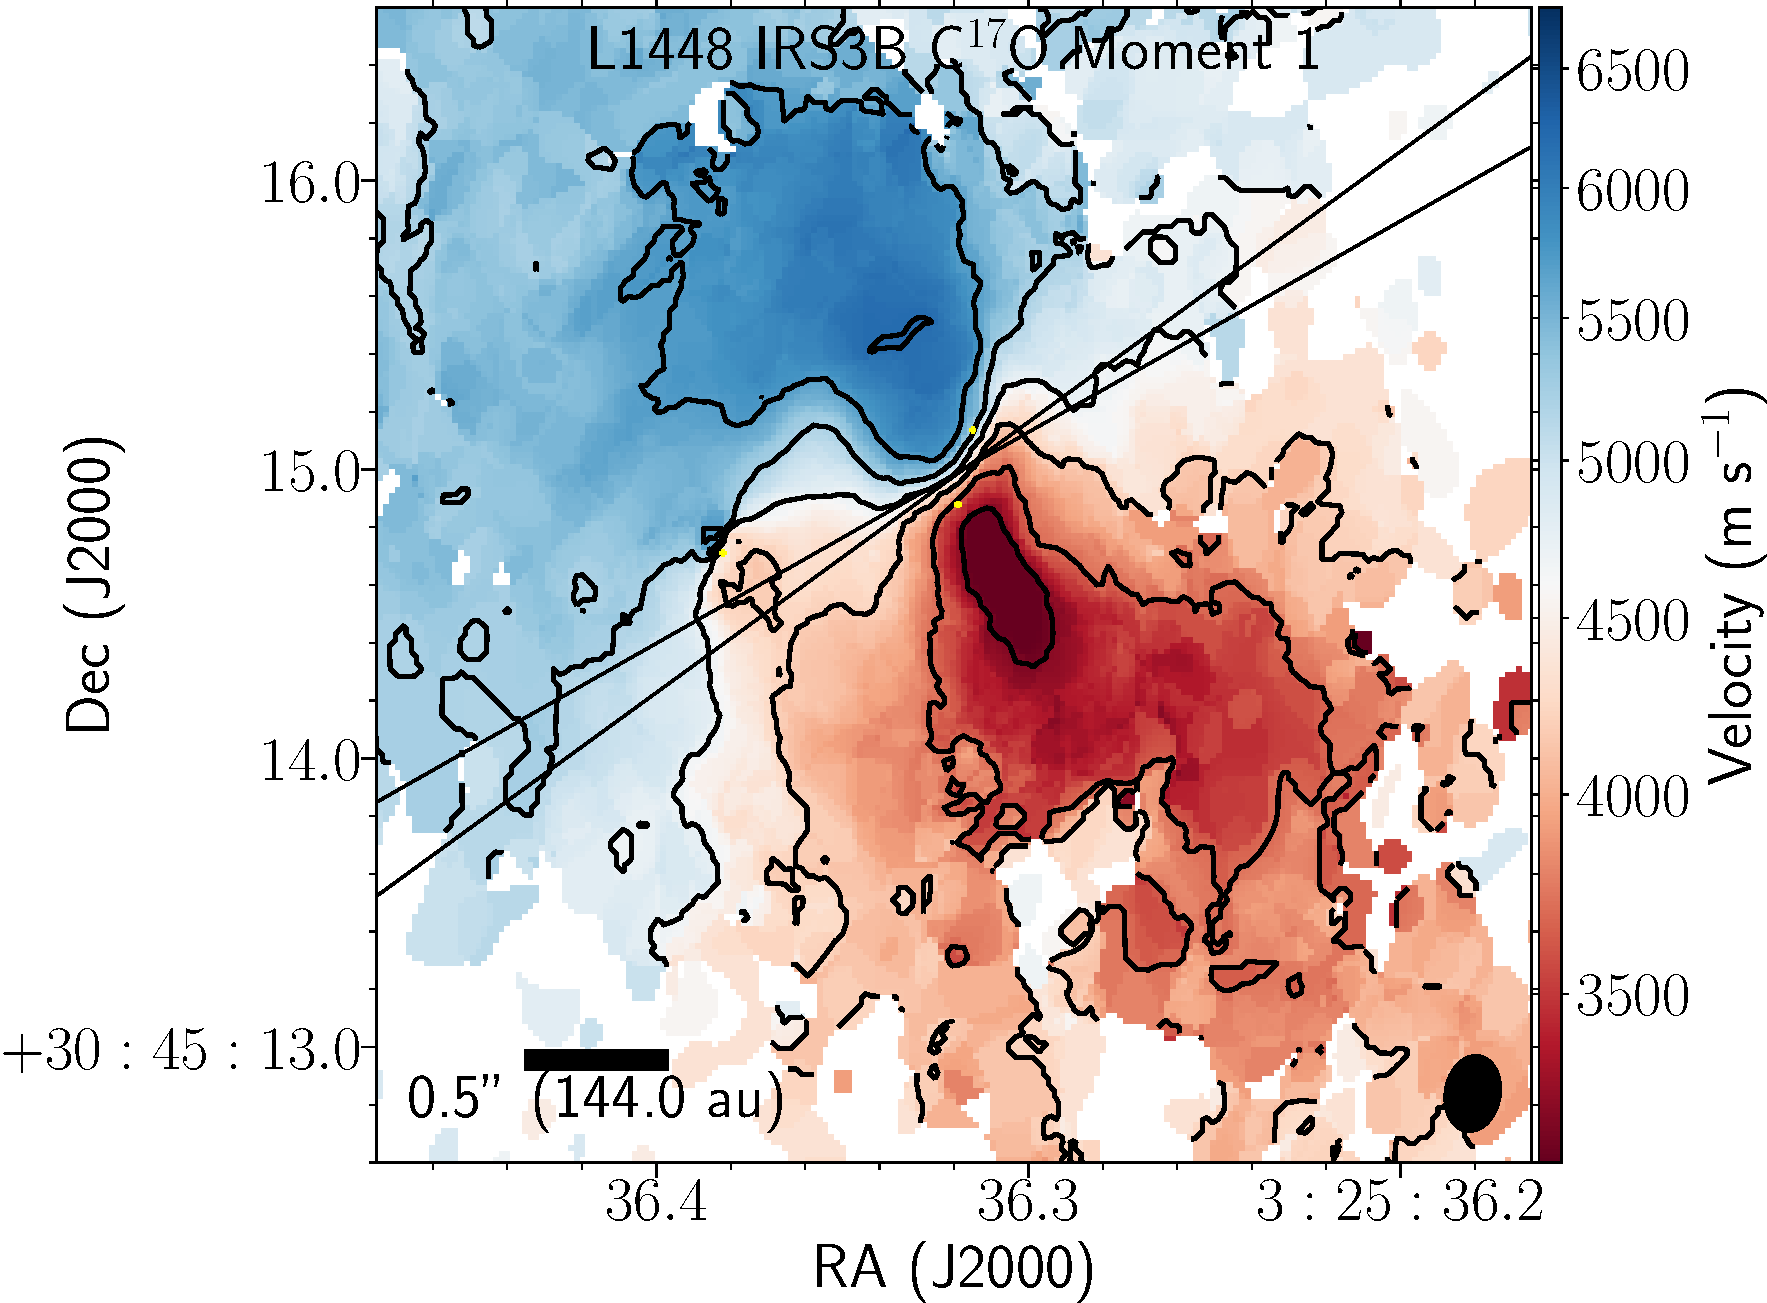
\includegraphics[width=0.5\textwidth]{img/L1448IRS3B_C17O_image_taper1500k_image_M1_fits.pdf}  % c17o
\end{center}
   \caption{\cso\space velocity-weighted moment 1 maps toward IRS3B over a selected range of velocities (1.27$\rightarrow$7.65~\kms) The \cso\space emission appears well ordered across the semi-major axis. The contours denote the 0.5~km~s$^{-1}$ velocity offsets from system velocity of 4.8~km~s$^{-1}$. The yellow markers indicate the three continuum sources. The black lines indicate the position angle of the minor disk estimates as given by the \pdspy\space fitting routine in Table~\ref{table:pvtable}, of $90+26.7^{+  1.8}_{-  2.9}$\deg. The \cso\space synthesized beam (\csobeam) is the bottom-right most ellipse.}\label{fig:irs3abc17omoment1}
\end{figure}

% figure will go here for pv cutout, 2 of them




% Figure 10
\begin{figure}[H]
\begin{center}
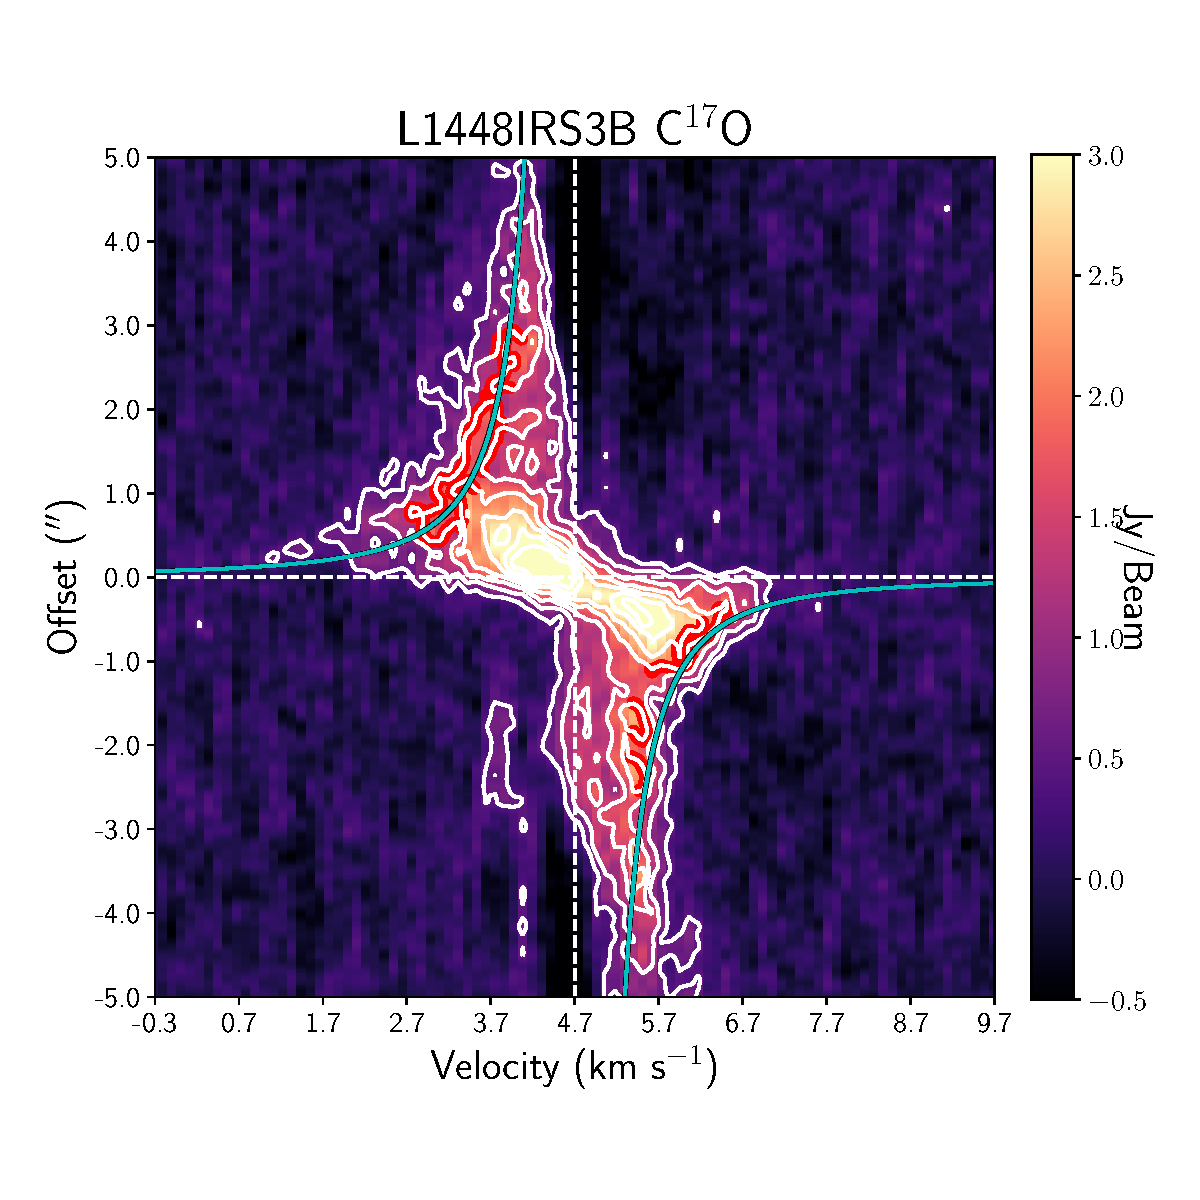
\includegraphics[width=0.49\textwidth]{img/irs3b_c17o_pv.pdf}
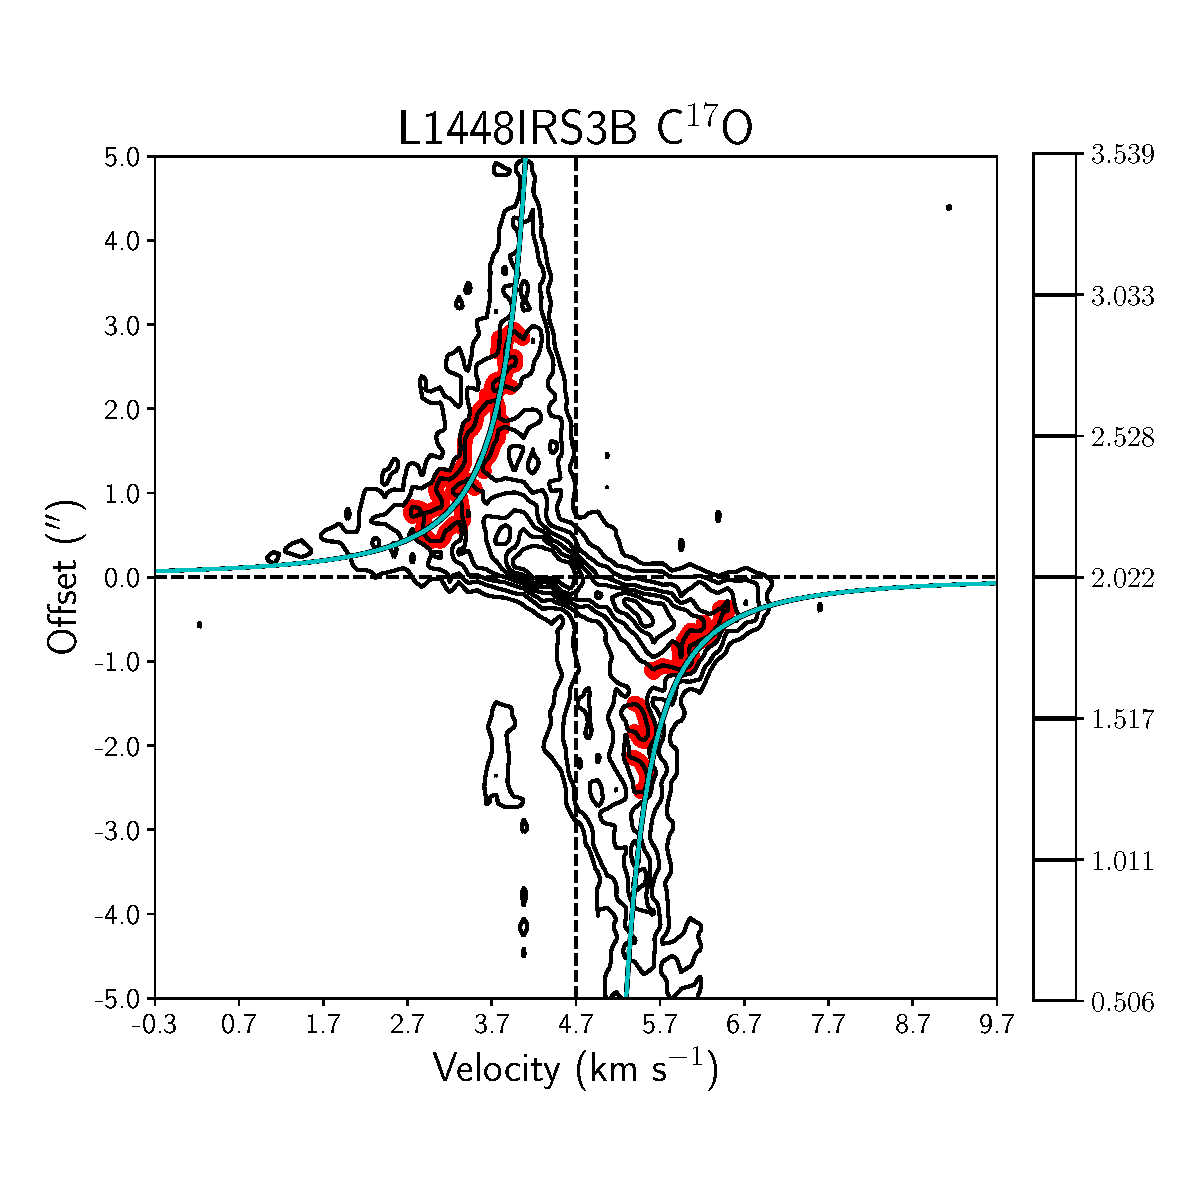
\includegraphics[width=0.49\textwidth]{img/PV-Diagram_L1448IRS3B_C17O_image_taper1500k_fit_xtr.pdf}
%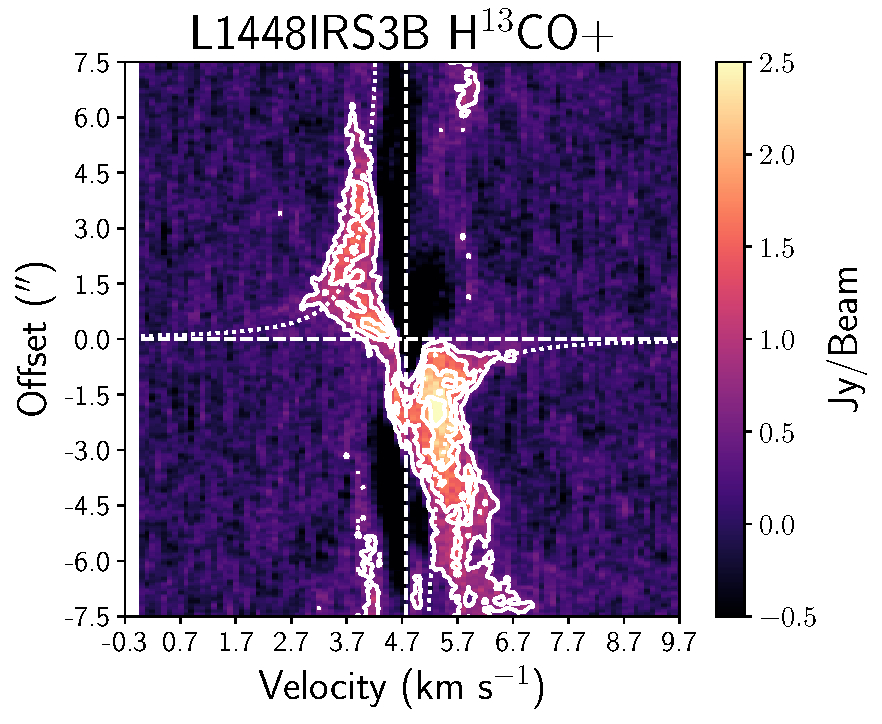
\includegraphics[width=0.33\textwidth]{img/PV-Diagram_L1448IRS3B_H13COp_image_taper1500k.pdf}
\end{center}
\caption{PV-diagrams of IRS3B generated at a position angle of 29\deg. \cso\space (left, middle) emission with the cyan lines corresponding to the fit of 1.15~\solm. The cyan line traces the median fit for numeric Keplerian orbital fit routine while the black lines represent 100 randomly sampled MCMC fits, used to estimate errors. The white/black contours trace regions starting from 3$\sigma$ at 2$\sigma$\space intervals, where $\sigma\approx$0.14~Jy~beam$^{-1}$. The red contours trace the regions selected for the MCMC fit which are defined as the 10 and 12$\sigma$. \htcop\space (right) demonstrates the data are not inconsistent with a 1.15~\solm\space protostar, however the emission is largely asymmetric and coupled with the envelope. The white contours trace regions starting from 3$\sigma$ at 2$\sigma$\space intervals, where $\sigma\approx$0.15~Jy.}\label{fig:l1448irs3b_c17o_pv}
\end{figure}




% Figure 7
\begin{figure}[H]
\begin{center}
   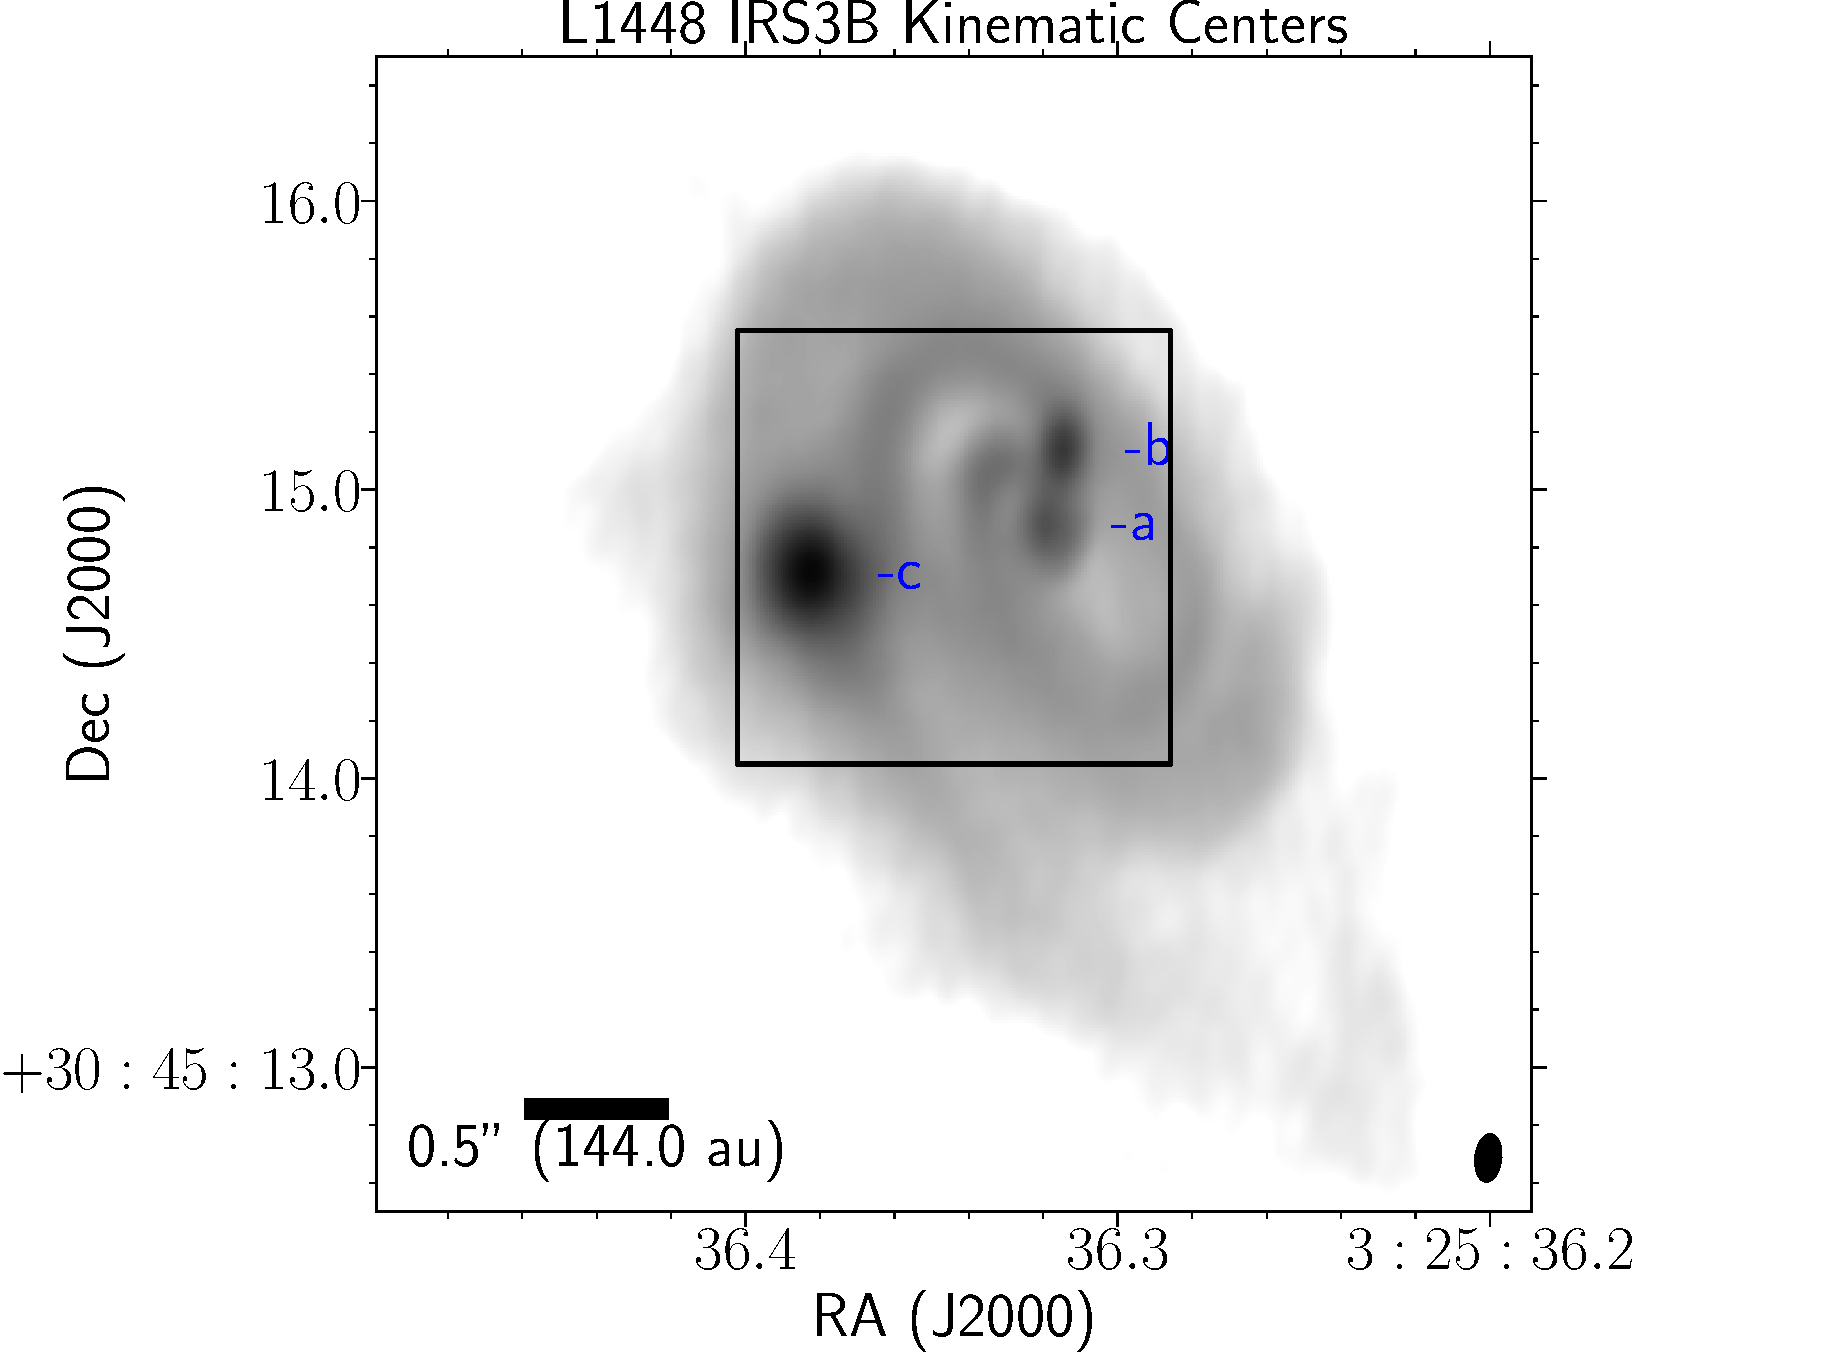
\includegraphics[width=0.48\textwidth]{img/L1448IRS3B_cont_robust05kincenters.pdf} % h13cn
   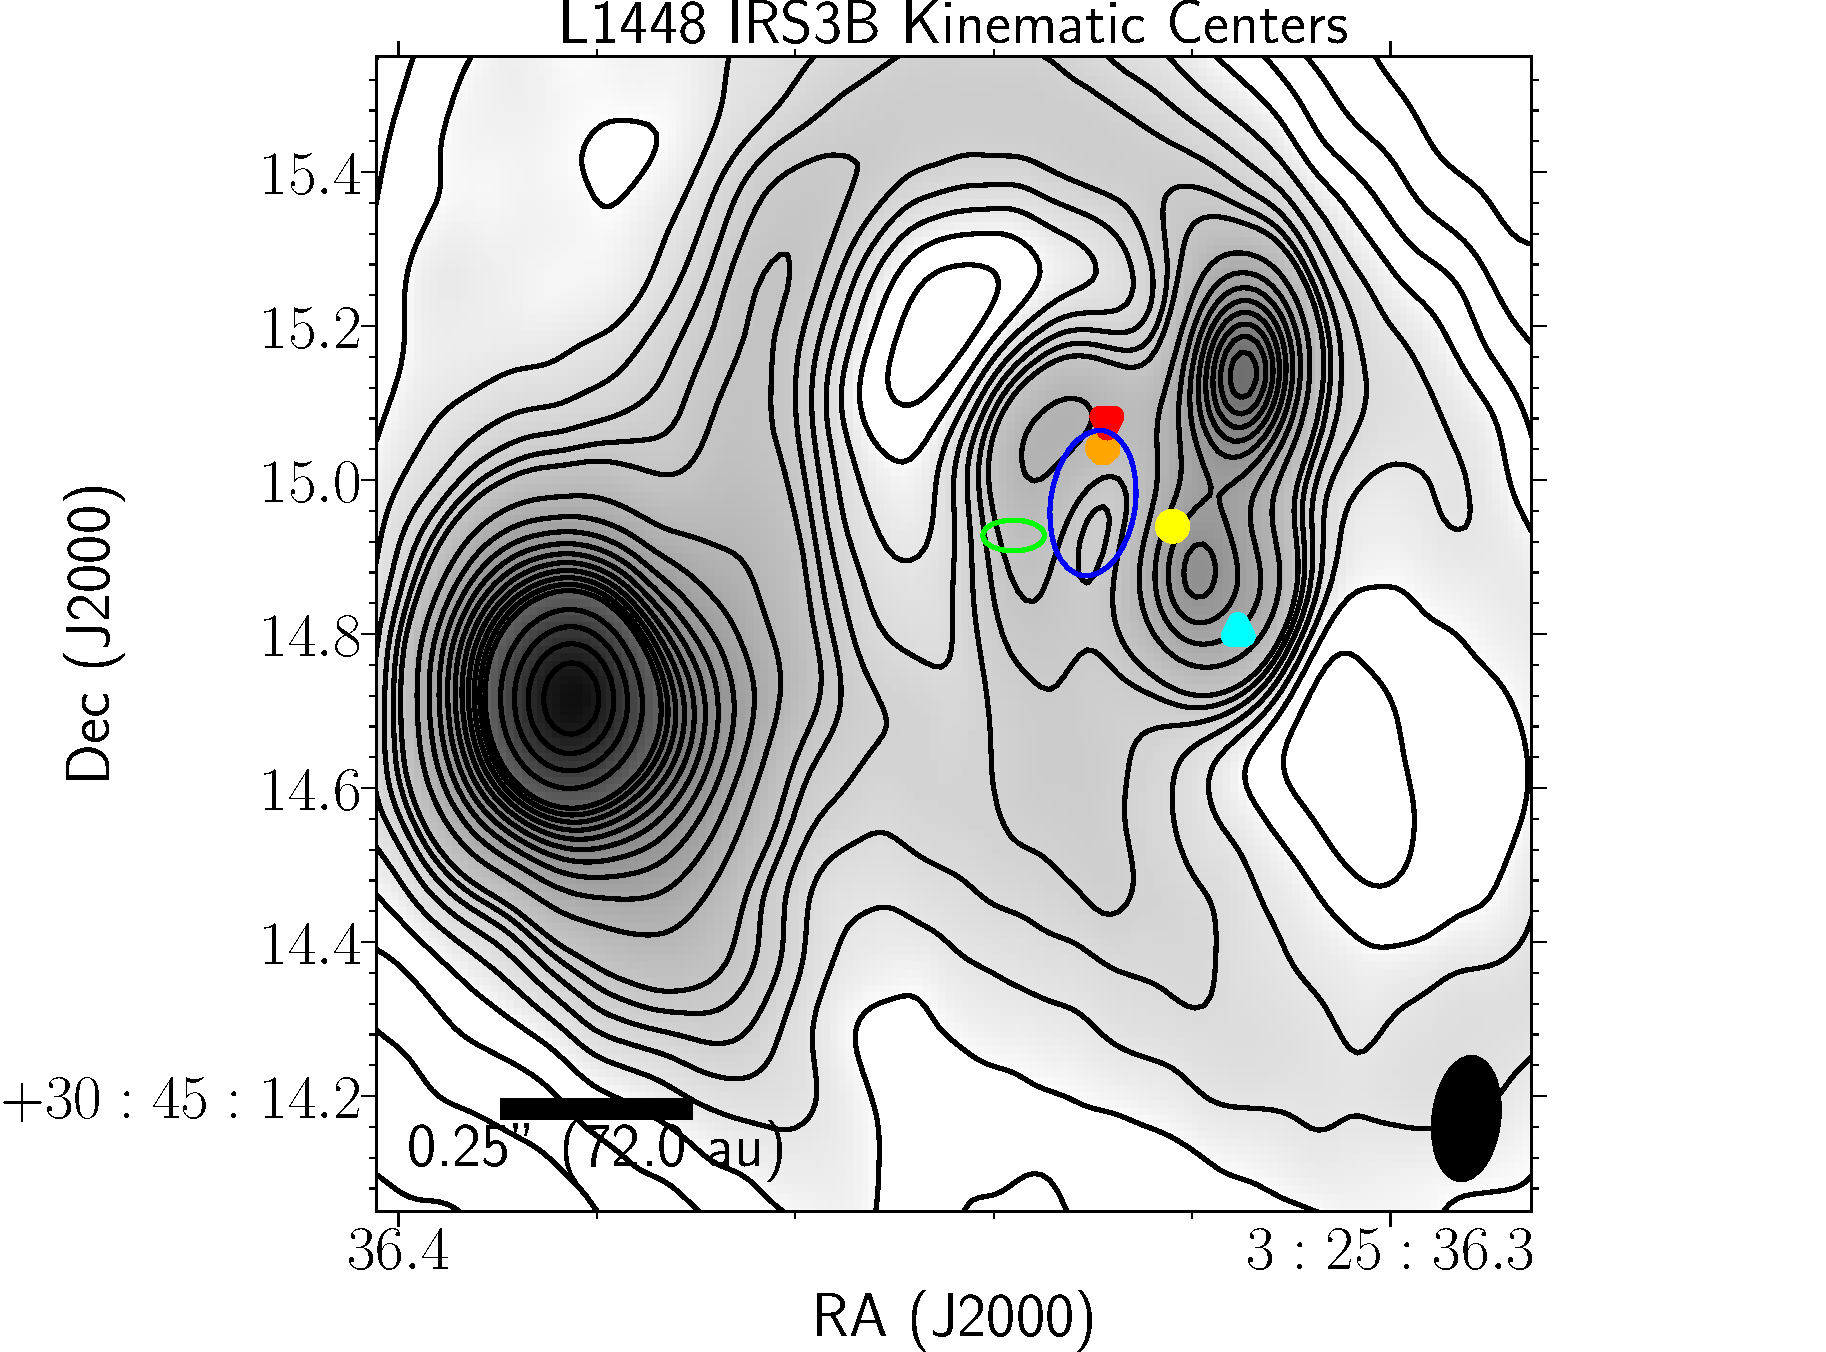
\includegraphics[width=0.48\textwidth]{img/L1448IRS3B_cont_robust05kincenters_zoom.pdf} % h13cn
\end{center}
   \caption{Positions of the various ``kinematic centers'' that have been fit from \cso\space emission at IRS3B in relation to continuum structure. The grayscale is the dust continuum from Figure~\ref{fig:zoomincont}. Left: The red colored texts detail the locations of continuum sources, presumed to be protostars. Right: A zoom in on the region indicated by the black rectangle in the left image. The red and blue triangles indicate the central Gaussian fit of the highest Doppler-shifted velocity emission with the yellow circle indicating the midpoint. The orange circle indicates the center that best constructs the PV diagram symmetrically. The green ellipse is the model Keplerian centroid fit with the respective error as indicated by the size of the ellipse (see Section~\ref{sec:kmodelresults}). The blue ellipse is the \cso\space beam (\csobeam) centered on the region of emission deficit for size comparison. The contours start at 10$\sigma$\space and iterate by 10$\sigma$\space with the 1$\sigma$~level starting at 8.5$\times10^{-5}$~Jy~beam$^{-1}$. The region of deficit, first identified in Figure~\ref{fig:zoomincont}\space is shown to be centered within the three various kinematic center fits and are marginally separated by less than a few beams.}\label{fig:kincenter}
\end{figure}




% figure 17 here

% Figure 16
\begin{figure}[H]
\begin{center}
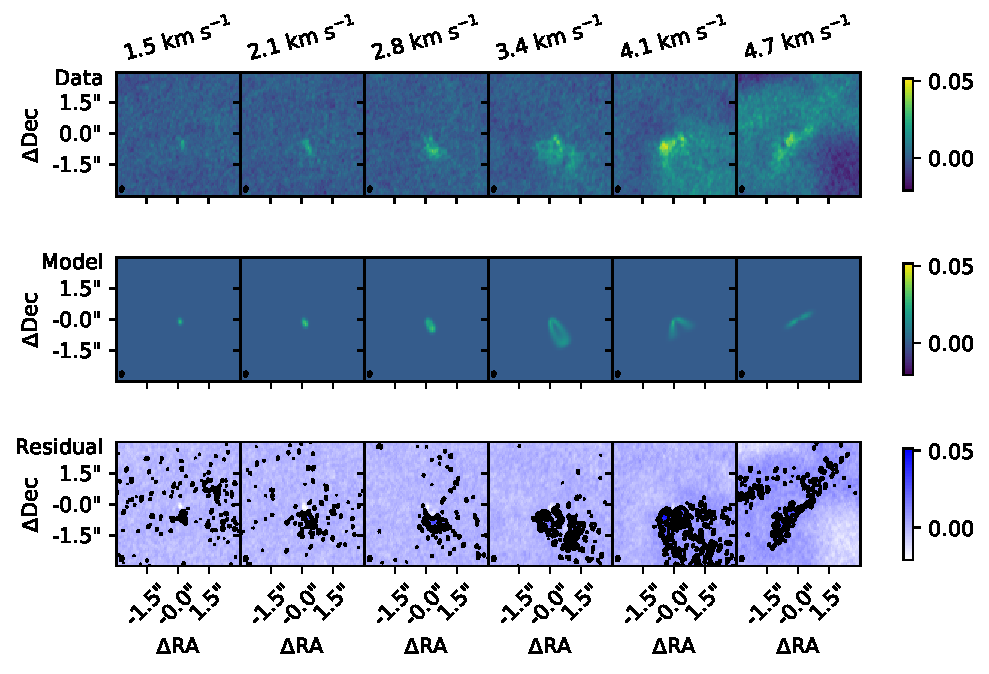
\includegraphics[width=0.49\textwidth]{img/Channelplot_irs3bplotblue_C17O.pdf}
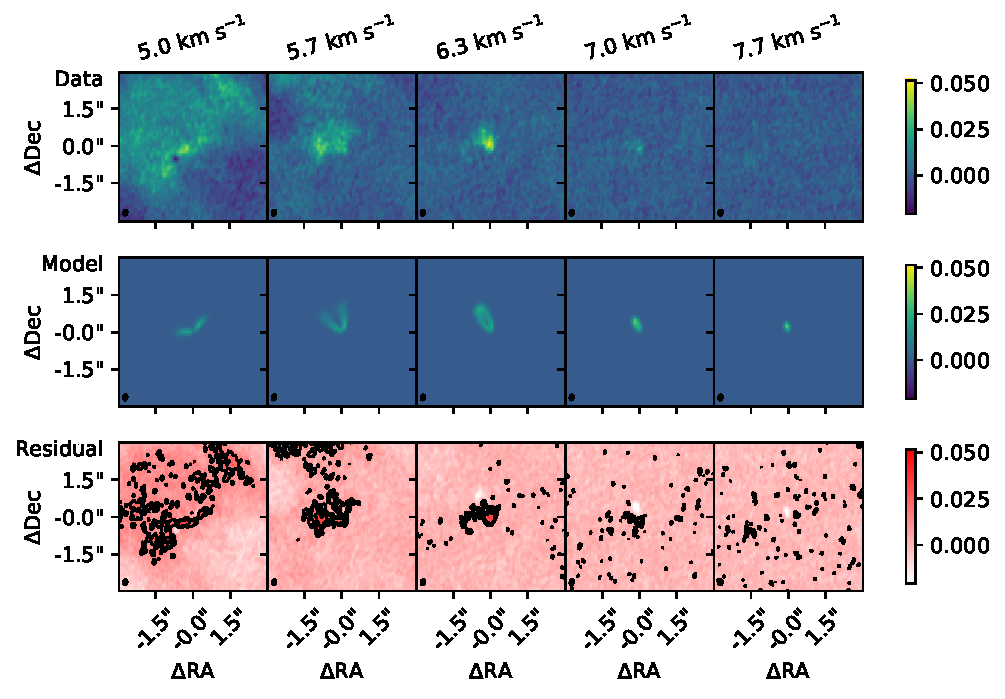
\includegraphics[width=0.49\textwidth]{img/Channelplot_irs3bplotred_C17O.pdf}
\end{center}
\caption{IRS3B Kinematic Model: A representative selection of channel maps that fit the model to the data. The left figure is the blue Doppler shifted emission while the right figure is the red Doppler shifted emission. The first row contours are the model contours, generated at the 2, 3, 5, and 10$\sigma$ level overlaid the data channels selected at the same velocity. The second row is the residual contours (2 and 3$\sigma$) overlaid the same data channels. System velocity is \ab4.8~km~s$^{-1}$. It should be noted the highly correlated structure visible in the residuals. This reflects an imperfect fit to the data given that the circumstellar disk itself is asymmetric.}\label{fig:c17o_res}
\end{figure}



% figure 21
\begin{figure}[H]
\begin{center}
%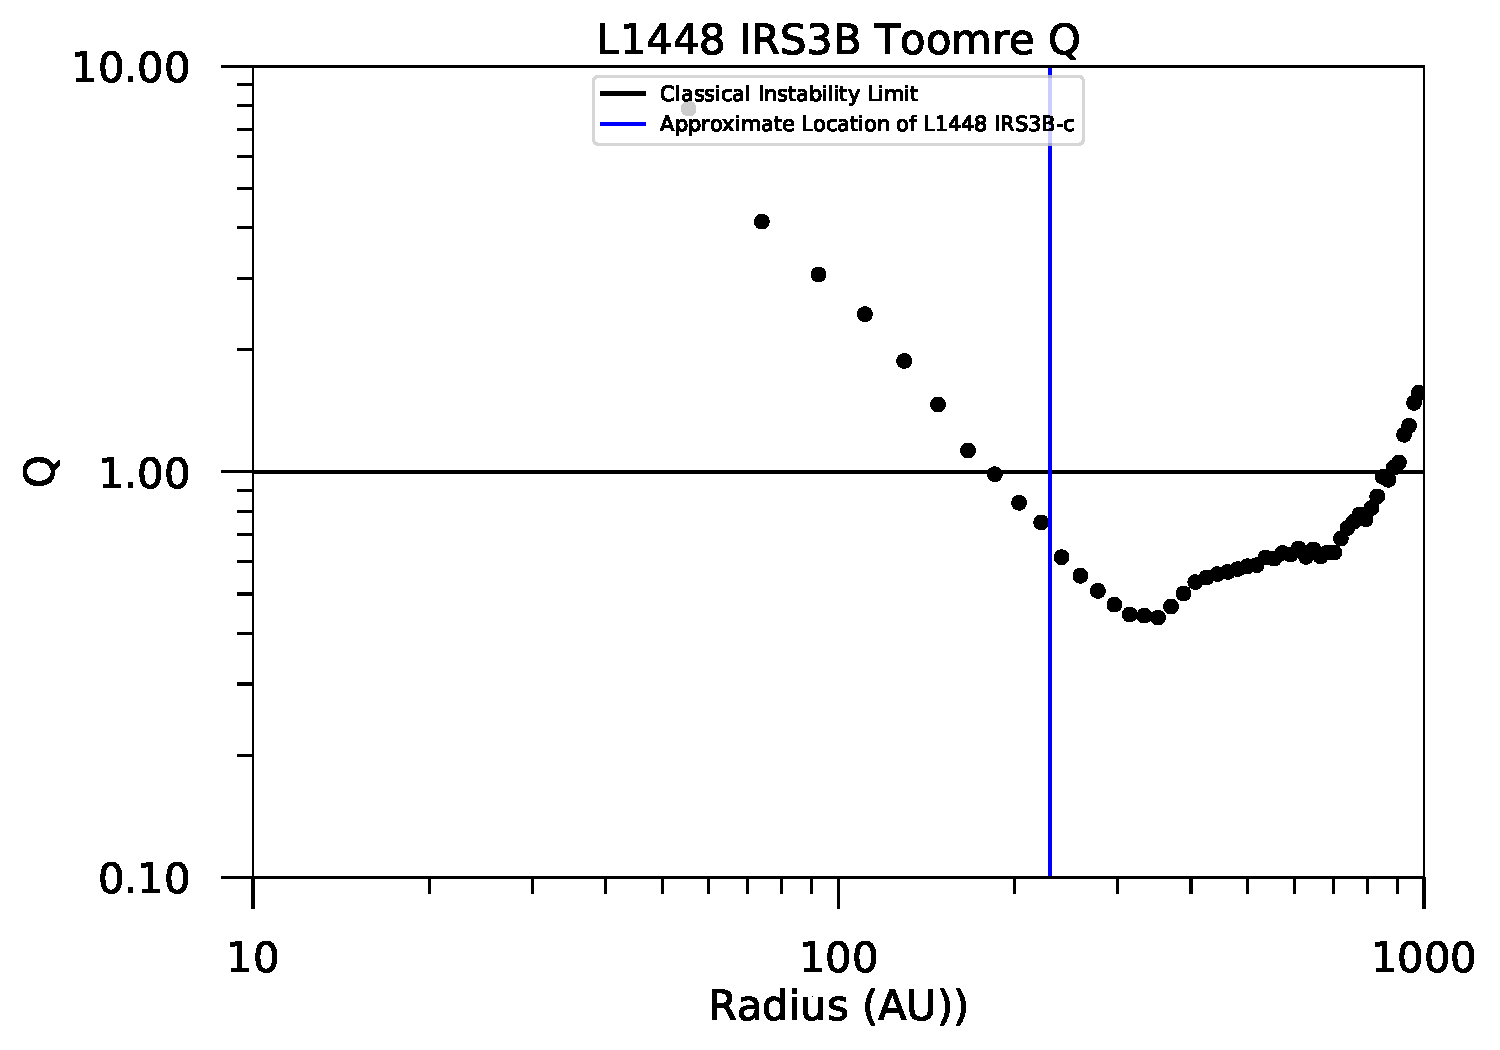
\includegraphics[width=0.48\textwidth]{img/L1448N-toomre-Q-linear-xsec-c17o_cont.pdf}
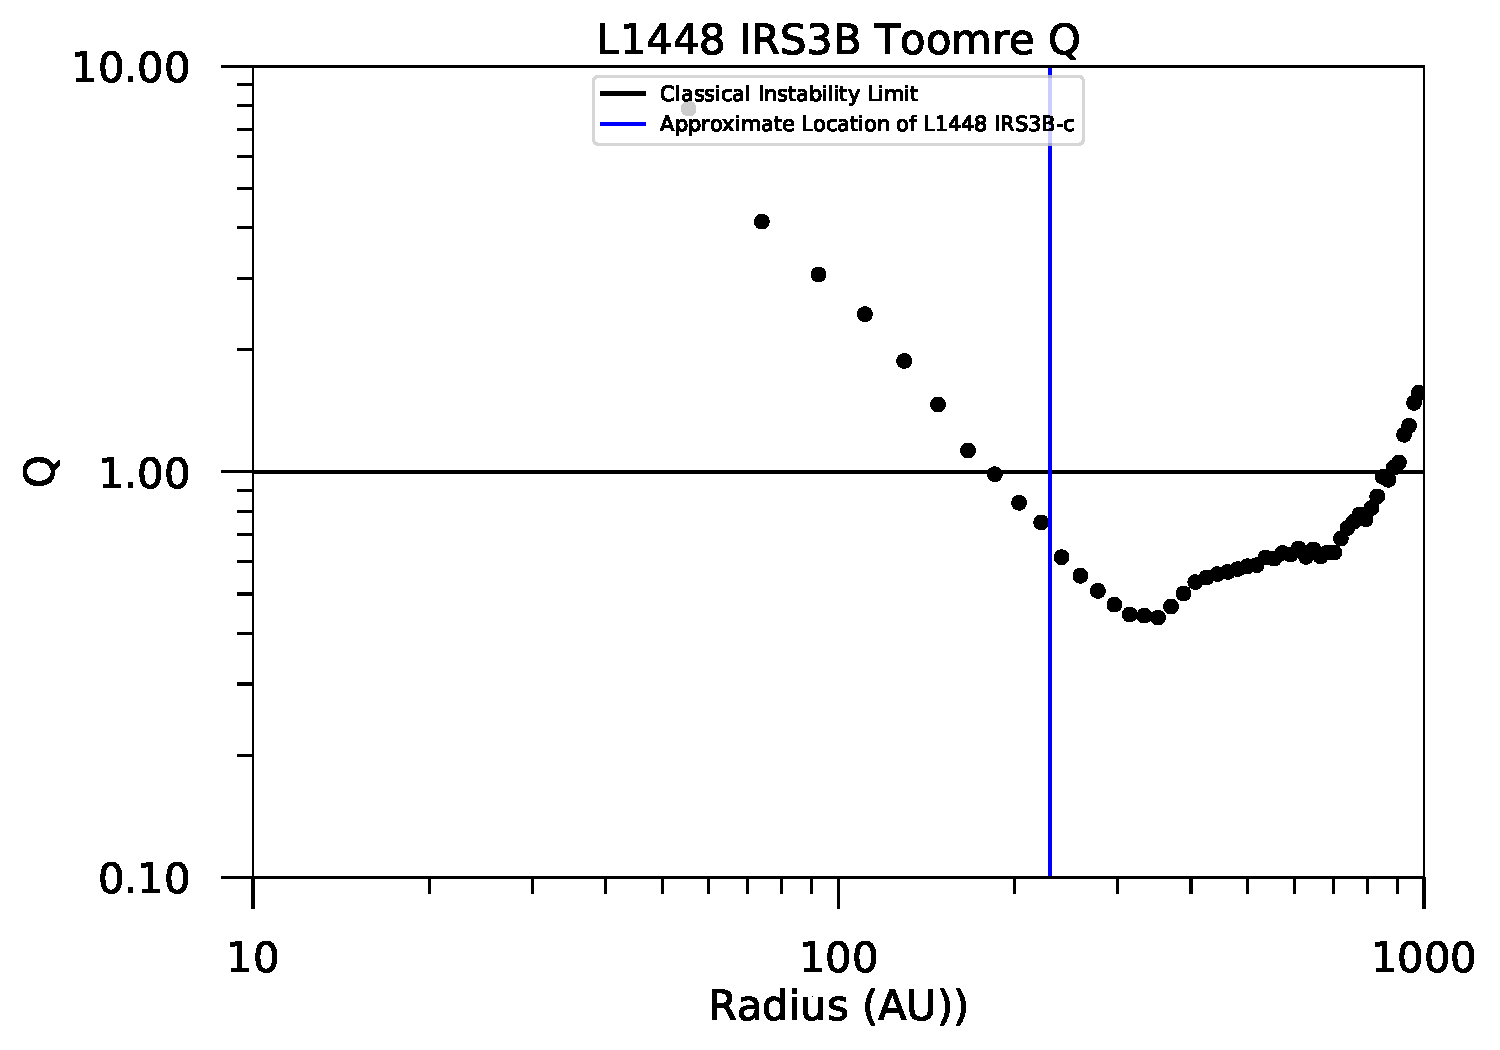
\includegraphics[width=0.49\textwidth]{img/L1448N-toomre-Q-linear-xsec-c17o_cont.pdf}
%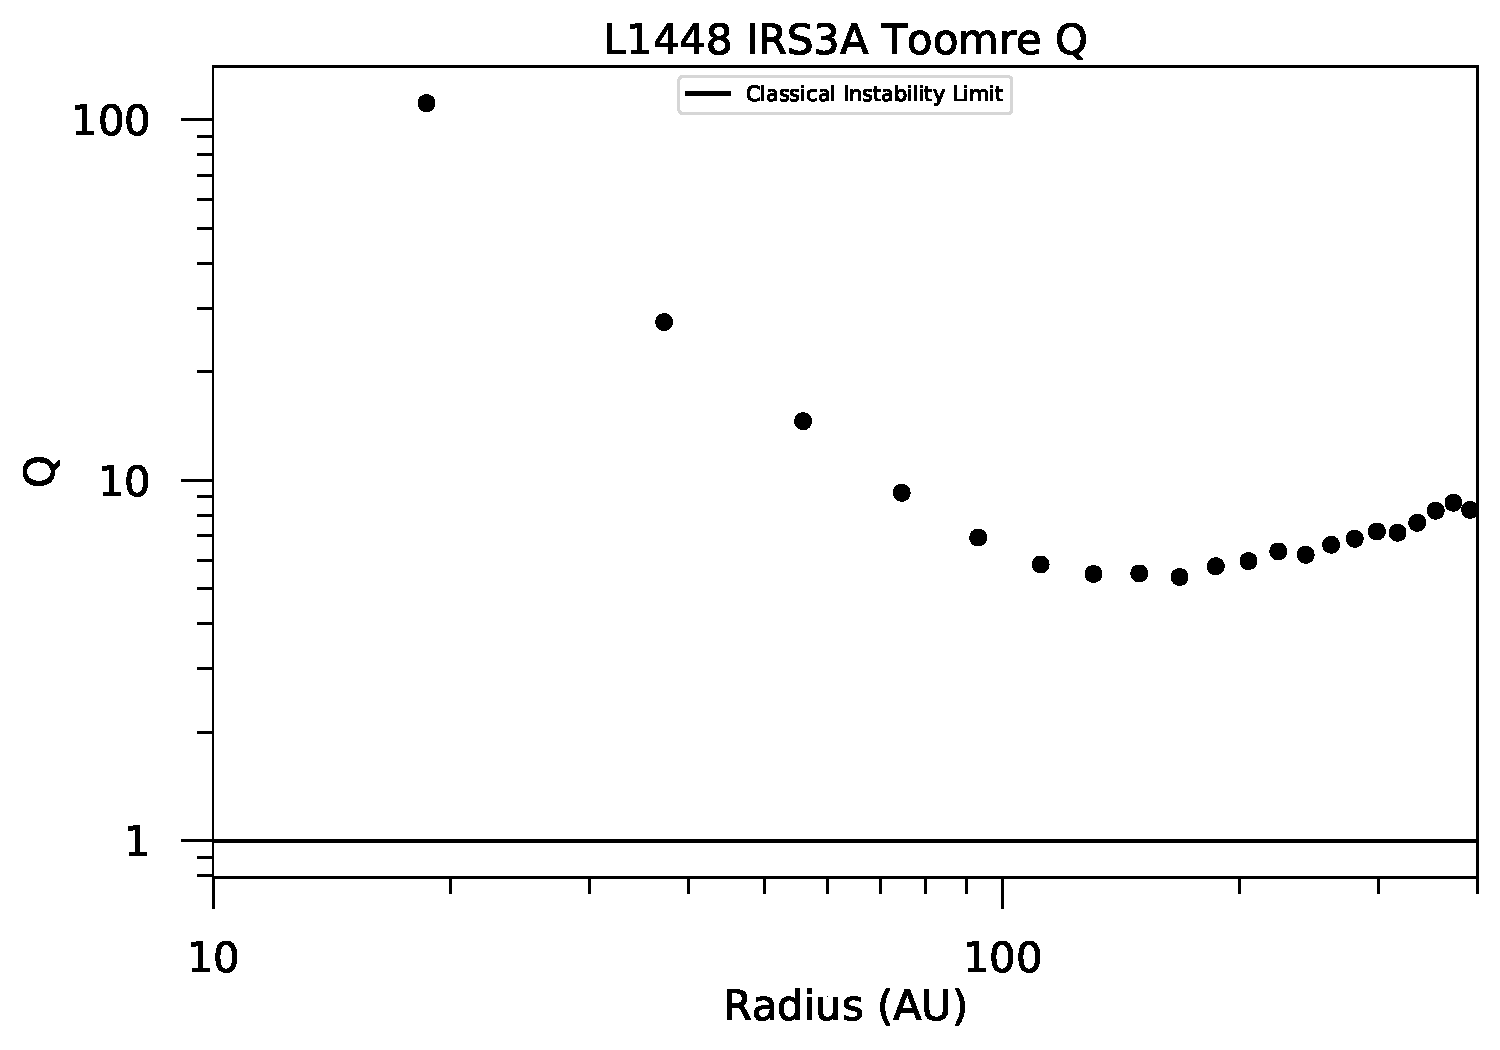
\includegraphics[width=0.49\textwidth]{img/L1448N-toomre-Q-linear-xsec-cont_robust-05_wide.pdf}
\end{center}   
\caption{Toomre Q parameter plotted as a function of deprojected radius for IRS3B (left) and IRS3A (right). The horizontal line indicates a Toomre Q parameter of one, at which the disk would be gravitationally unstable. As indicated, the IRS3B disk Toomre Q parameter drops below 1 at a radius of \ab120~AU. The vertical line corresponds to the deprojected radius of IRS3B-c. The observed spiral arms also become most prominent at R $>$100~AU, where Toomre~Q approaches 1. The circumstellar disk of IRS3A is much less massive than IRS3B, coupled with a more massive protostar, the disk is more stable against gravitational instabilities.}\label{fig:irs3btoomreq}
\end{figure}

